\subsection{Mikrocontroller}\label{subsec: Mikrocontroller}
Die Auswahl des Mikrocontrollers, ist so ausgefallen, dass dieser für Sensor wie auch für Aktor-Layout geeignet ist. Das Hauptkriterium der Wahl basiert auf der Kommunikation. Der Mikrocontroller von der chinesischen Firma Espressif Systems ist ein Robuster Chip, welcher für industrielle Umgebungen geeignet ist und in Betriebstemperaturen von -40 °C bis +125 °C zuverlässig arbeitet. Der Stromverbrauch kann zwischen verschiedenen Leistungsmodi gewählt werden, so kann während dem Betrieb eine dynamische Leistungsskalierung bewerkstelligt werden. ESP32 Module sind mit integrierten Antennen, Leistungsverstärkern und rauscharmen Empfangsverstärkern hochintegriert. Schnittstellen wie SPI, I2C, UART, WiFi und Bluetooth sind vorhanden.\\
WiFi:
Arbeitet mit dem Standart 802.11b/g/n und 802.11 2,4 GHz bis zu 150 Mbit/s. 4 Virtuelle Wi-Fi interfaces und Soft AP \\
Bluetooth:
Kompatibel mit Bluetooth v4.2 BR/EDR und BLE-Spezifikationen. Sender Klasse 1, Klasse 2 und Klasse 3 ohne externen Leistungsverstärker. Hochgeschwindigkeits-UART HCI, bis zu 4 Mbits/s.\\
CPU und Memory:
Modell abhängig, wobei das Modell ESP-WROOM-32E, mit der Chip Bezeichnung D0WD -V3 betrachtet wird. Dual-Core 32-bit, Flash 4-16 MB, 448 KB ROM, 520 KB SRAM, 16 KB SRAM in RTC. \\
Prozessor:
Tensilica Xtensa LX6 240 MHz\\
Clocks und Timers:
Interner 8 MHz-Oszillator mit Kalibrierung. Externer Quarzoszillator 2 MHz bis 40 MHz. Zwei Timer Gruppen 2x 64-bit Timer mit je einem Haupt Watchdog.\\
Erweiterte Peripherieschnittstellen:
12-bit SAR ADC bis zu 18 Kanäle, 2x b-bit D/A Wandler, 10x touch Sensoren, Temperatursensor, 4x SPI, 2x I2S, 2x I2C 3x UART.\\
Sicherheit:
Alle unterstützten Sicherheitsfunktionen des IEEE 802.11-Standards, einschließlich WFA, WPA/WPA2 und WAPI\\
Unterstützung bei der Entwicklung:
SDK Firmware für schnelle on-line Programmierung und open Source toolchains basiert auf GCC.\\
Kosten bei Mouser:\\
356-ESP32WROOM-32D 3,71 CHF/Stück
\subsubsection{ADC} \label{ADC}
Der ADC des ESP32 verhält sich nicht liniear, was zu Problemen führen kann. In der Grafik \ref{pic: ESP32_Kurve} ist zu erkennen, dass der ADC nur bei grösser als U = 0.17\,V und kleiner als 3\,V überhaupt brauchbar ist, dazu kommt, dass ab 2.5\,V der ADC nichtliniear ansteigt. Die Lösung, welche hier verwendet wurde, war eine Linearisierung im Bereich von  0.2\,V bis 2.5\,V was zur Geradengleichung geführt hat. Die Daten stammen aus dem Internet. Diese ist somit mit Vorsicht zu bewerten, es wurden für den Sensor- und Aktorbaustein besser passende Geradengleichungen verwendet, eine für die Temperaturmessung und eine für die analogen Eingänge. Ebenso gibt es noch weitere Probleme mit der ADC-Messung, dazu mehr im Kapitel \ref{Verbesserungen} Verbesserungen.

\begin{align}
ADC = 1253.1\,frac{1}{V}\cdot U - 218.54 \label{ADC_Kurve} \\
U = 0.000798 + 0.174 \label{U_kurve}\\
\end{align}

\begin{figure}[h!]
	\centering
	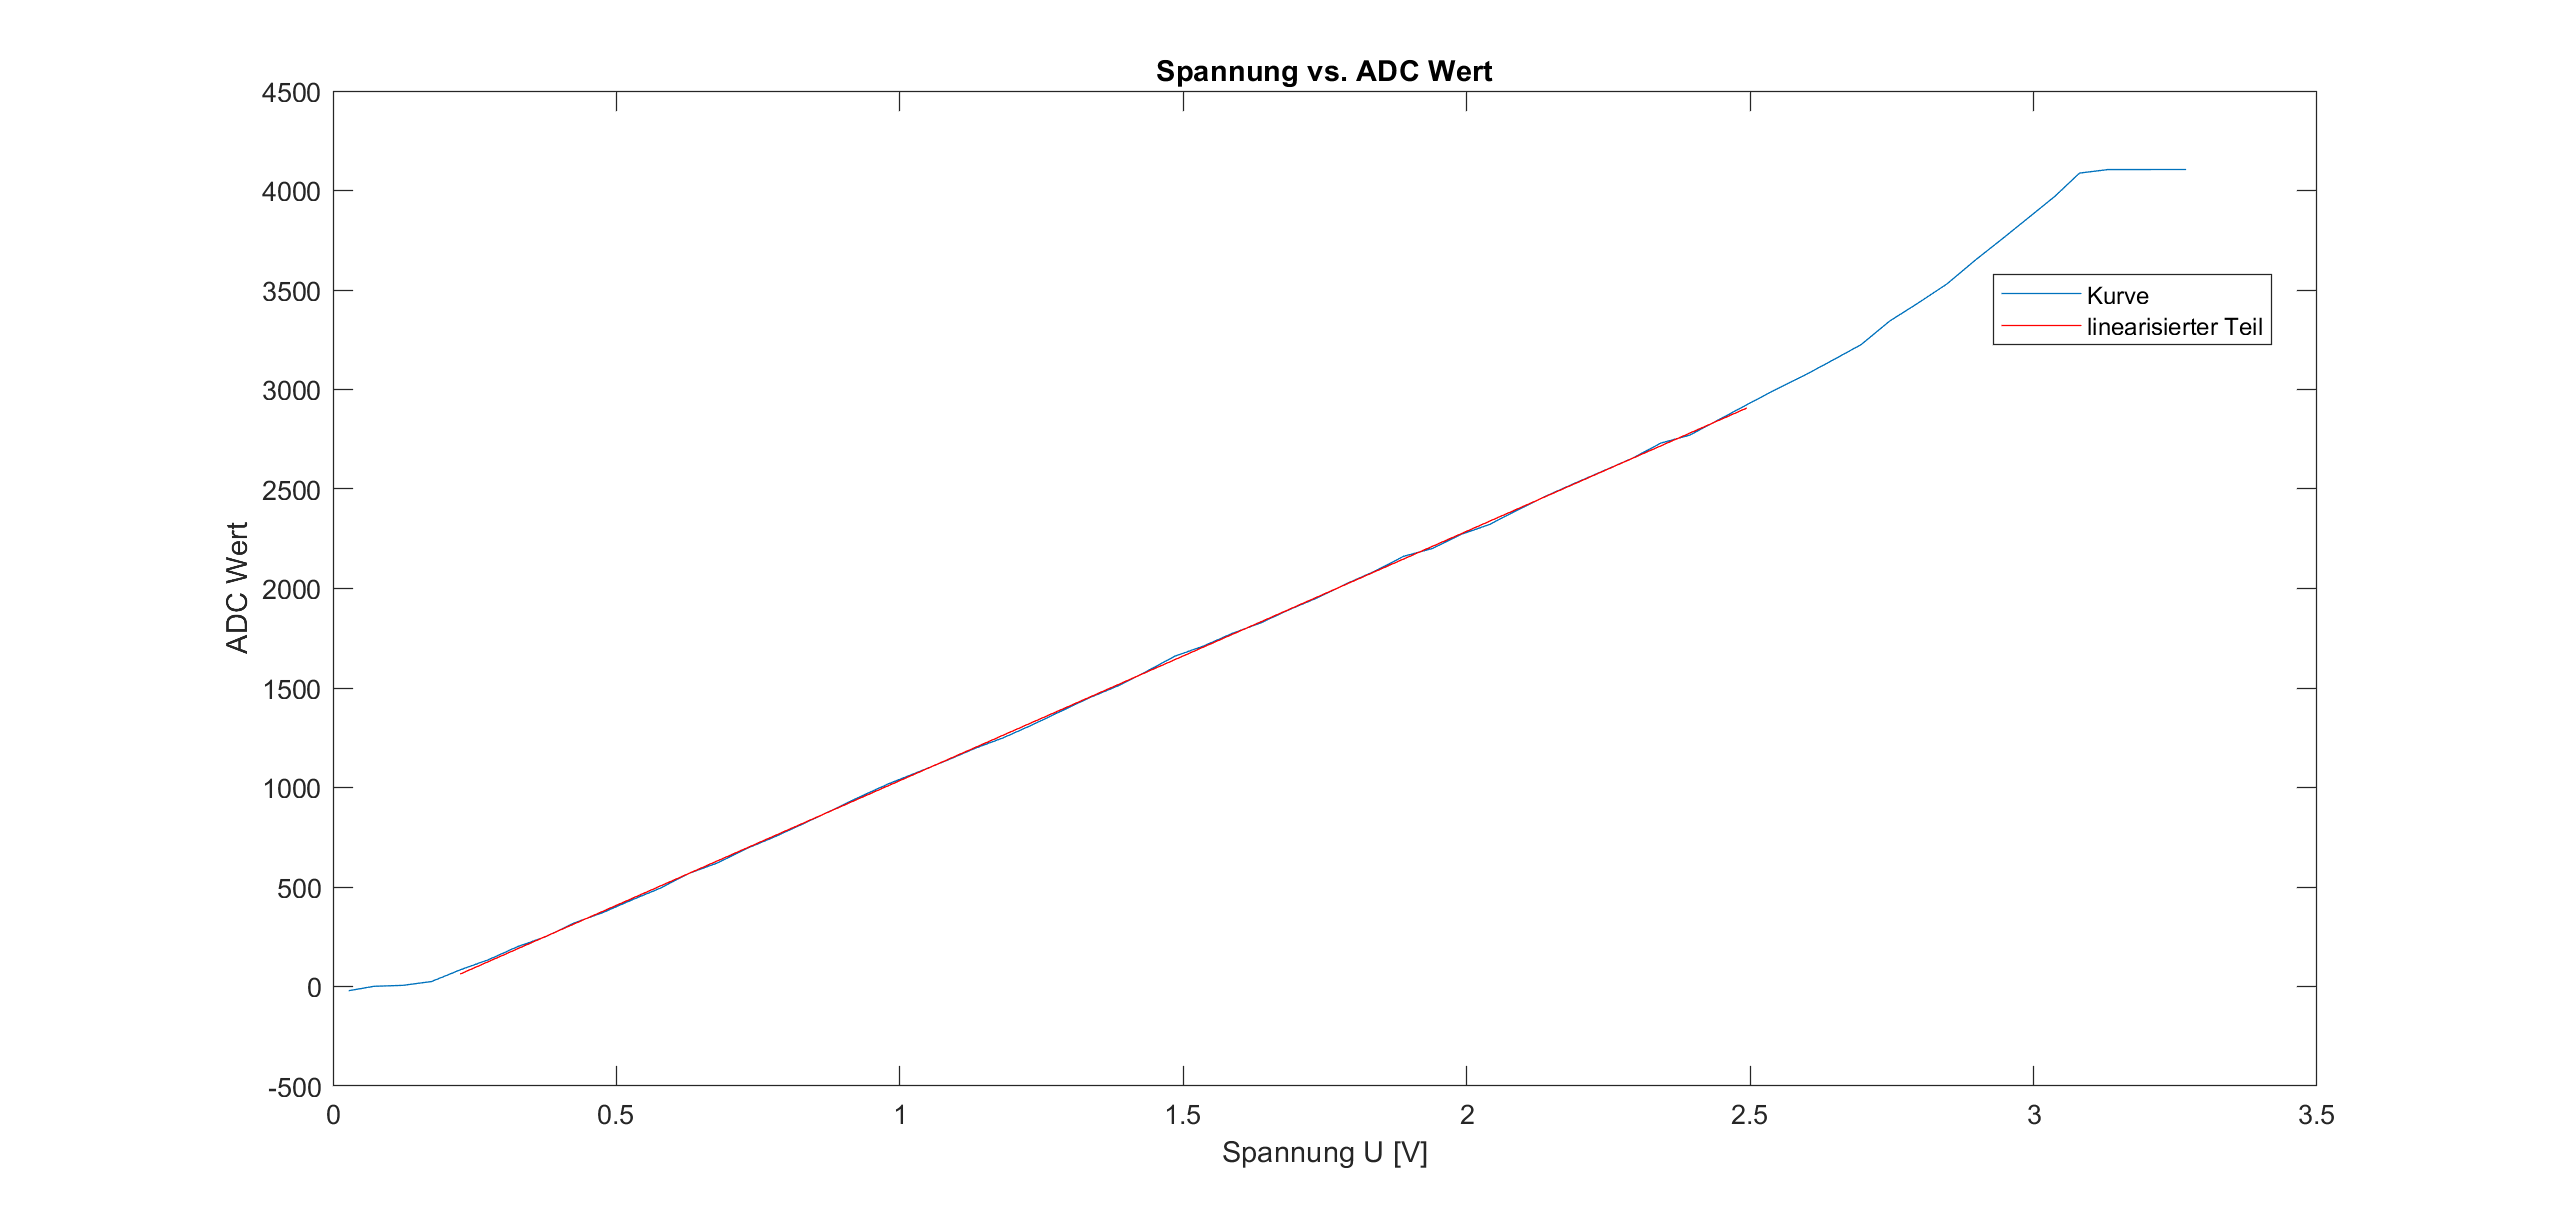
\includegraphics[width=\textwidth]{graphics/ESP32_Kurve.png}
	\caption{ESP32 Kurve, Daten aus Grafik von \cite{randomnerdtutorials_esp32_2019}}
	\label{pic: ESP32_Kurve}
\end{figure}

